





% !TEX TS-program = pdflatex
% !TEX encoding = UTF-8 Unicode

% This is a simple template for a LaTeX document using the "article" class.
% See "book", "report", "letter" for other types of document.

\documentclass[11pt]{article} % use larger type; default would be 10pt

\usepackage[utf8]{inputenc} % set input encoding (not needed with XeLaTeX)

%%% Examples of Article customizations
% These packages are optional, depending whether you want the features they provide.
% See the LaTeX Companion or other references for full information.

%%% PAGE DIMENSIONS
\usepackage{geometry} % to change the page dimensions
\geometry{a4paper} % or letterpaper (US) or a5paper or....
% \geometry{margin=2in} % for example, change the margins to 2 inches all round
% \geometry{landscape} % set up the page for landscape
%   read geometry.pdf for detailed page layout information

\usepackage{graphicx} % support the \includegraphics command and options

% \usepackage[parfill]{parskip} % Activate to begin paragraphs with an empty line rather than an indent

%%% PACKAGES
\usepackage{booktabs} % for much better looking tables
\usepackage{array} % for better arrays (eg matrices) in maths
%\usepackage{paralist} % very flexible & customisable lists (eg. enumerate/itemize, etc.)
\usepackage{verbatim} % adds environment for commenting out blocks of text & for better verbatim
\usepackage{subfig} % make it possible to include more than one captioned figure/table in a single float
% These packages are all incorporated in the memoir class to one degree or another...

%%% HEADERS & FOOTERS
\usepackage{fancyhdr} % This should be set AFTER setting up the page geometry
\pagestyle{fancy} % options: empty , plain , fancy
\renewcommand{\headrulewidth}{0pt} % customise the layout...
\lhead{}\chead{}\rhead{}
\lfoot{}\cfoot{\thepage}\rfoot{}

%%% SECTION TITLE APPEARANCE
\usepackage{sectsty}
\allsectionsfont{\sffamily\mdseries\upshape} % (See the fntguide.pdf for font help)
% (This matches ConTeXt defaults)

%%% ToC (table of contents) APPEARANCE
\usepackage[nottoc,notlof,notlot]{tocbibind} % Put the bibliography in the ToC
\usepackage[titles,subfigure]{tocloft} % Alter the style of the Table of Contents
\renewcommand{\cftsecfont}{\rmfamily\mdseries\upshape}
\renewcommand{\cftsecpagefont}{\rmfamily\mdseries\upshape} % No bold!

%%% END Article customizations
\usepackage{url}
\usepackage[spanish]{babel}
\usepackage{listings} 
%%% The "real" document content comes below...

\title{Recolección de Basura en C}
%\date{} % Activate to display a given date or no date (if empty),
         % otherwise the current date is printed 
         
\author{Edinson Sánchez\\Kevin Filella\\Adrian Aguilar}

\begin{document}
\maketitle

%----------------------------------------------------------------------------------------
%	TABLE OF CONTENTS
%----------------------------------------------------------------------------------------

%\setcounter{tocdepth}{1} % Uncomment this line if you don't want subsections listed in the ToC

\newpage
\tableofcontents
\newpage

\section{Introducción}
	En lenguajes de programación, un recolector de basura tiene como objetivo el de gestionar la memoria de un programa informático. La memoria debe ser gestionada de tal forma que se puedan reservar espacios en memoria para su uso, se puedan liberar espacios en memoria anteriormente reservados, se puedan compactar espacios de memoria libres y consecutivos, y se pueda llevar cuenta de los espacios libres y utilizados en la memoria.

	Como es de conocimiento para muchos, el lenguaje C no incorpora un método de gestión de memoria automático, como lo hacen lenguajes de programación como Java, C Sharp, entre otros. Esto brinda a los programadores un set de ventajas y desventajas a la hora de programar.

	En este documento, discutiremos sobre varios métodos populares que han sido creados, en forma de librerías, para brindarle al lenguaje C esta muy importante característica. Asimismo, discutiremos sobe las ventajas y desventajas de tener un recolector de basura automático y gestionar la memoria manualmente.

\section{Métodos}

\subsection{Boehm-Demers-Weiser Garbage Collector}
	El método de recolección de basura de la librería Boehm GC consiste en dos fases; primero, se realiza un escaneo de toda la memoria activa para marcar bloques en desuso; después, la fase de barrido se hace cargo de mover todos los bloques marcados (de la primera fase) a la lista de bloques libres. Estas dos fases pueden ser, y usualmente son, ejecutadas aparte para mejorar el tiempo de respuesta de la librería.

	El algoritmo del Boehm GC es generacional, ya que se enfoca en buscar memoria libre en los bloques más nuevos. Esto se basa en la idea de que los bloques más viejos tienen mayor tiempo de uso; por consecuencia, los bloques más recientes tienen un tiempo de uso reducido y deben ser liberados con mayor frecuencia. Este algoritmo también es conservativo, ya que también se debe encargar de asumir cuales variables son punteros a datos dinámicos y cuales simplemente se ven de esa forma.

	La librería Boehm GC viene en forma estática o dinámica, es fácil de instalar, y su uso es permitido en los lenguajes C y C++. Para utilizar la librería en programas en C que ya utilizan malloc(), calloc(), realloc(), o free(), simplemente se deben redefinir las funciones como se ve a continuación:
\lstset{language=C}          % Set your language (you can change the language for each code-block optionally)

\begin{lstlisting}[frame=single]  % Start your code-block
#define malloc(x) GC_malloc(x)
#define calloc(n,x) GC_malloc((n)*(x))
#define realloc(p,x) GC_realloc((p),(x))
#define free(x) (x) = NULL
\end{lstlisting}

\subsection{Doug Lea's Malloc}
 Doug Lea's Malloc
\subsubsection{Introducción}
Dlmalloc lleva en uso desde 1987 y es la versión estándar de malloc() y free() en muchos ambientes, por lo tanto su confiabilidad es muy alta.
La “Memory allocator library  ” de Doug Lea es una librería estándar que empezó a escribirse en 1987, normalmente se la conoce como dlmalloc.
Dlmalloc es una librería abierta cuyo código puede ser obtenido en ftp://g.oswego.edu/pub/misc/malloc.c. 
Debido a esto el uso de esta librería es de uso extendido y general. Incluso sirve como la versión nativa default de la implementación de malloc y free en algunas versiones de Linux. Esta librería normalmente hace overwrite al malloc nativo en varios paquetes de software comunes y además se usa en varios ambientes de PC así como en sistemas embebidos. 
\subsubsection{Metas}

Estas son las metas propuestas en el desarrollo de la dlmalloc.

Maximizar Compatibilidad, en particular obedecer las convenciones ANSI/POXI

Maximizar Portabilidad, es decir, depender lo menos posible de características dependientes del Sistema como system calls, ademas de conformarse a todos los constraints conocidos del Sistema.

Minimizar el Espacio. Esto se refiere a que el allocator no debe desperdiciar memoria. Debe obtener la mínima cantidad de memoria que sea posible y mantener la misma de tal manera que se minimiza la fragmentación de la misma.

Minimizar el Tiempo. Quiere decir que malloc(), free() y realloc() deben ser lo mas rapidas posibles en cuanto a su tiempo promedio de ejecución.

Maximizar Afanabilidad (Tunability). Las características y comportamientos opcionales de dlmalloc deben poder ser controlados por el usuario, ya sea estática o dinámicamente.

Maximizar Localidad. Se ubican pedazos de memoria que se utilizan típicamente juntos en cercanía unos de otros. Esto ayuda a minimizar la cantidad de miss de páginas y de cache durante la ejecución.




Detección de Errores. Aunque no es posible que esta librería de uso general sirva también como una librería de detección de errores de memoria como Purify, si debe proveer algún medio para detector corrupción de memoria debido a sobre-escritura, múltiples frees, etc..

Minimizar Anomalías. Si el allocator es configurado usando los valores default debería funcionar bien en una amplia gama de aplicaciones tales como aplicaciones GUI, compiladores, interpretadores, IDEs , programas con intensive networking, paquetes gráficos, web browsers , etc …

\subsubsection{Algoritmos}

La Dlmalloc usa dos algoritmos como base para su funcionamiento. Boundary y Binning, los cuales han permanecido aproximadamente iguales desde sus primeras versiones.
Boundary Tags(Tags de frontera)\\

Los pedazos de memoria llevan consigo el size tanto al principio como al final del mismo, lo que permite la implementación de dos capabilities muy importantes.\\
•	Dos pedazos de memoria contiguos y sin utilizar pueden juntarse en un pedazo más grande, esto minimiza la fragmentación y el número de pedazos pequeños inutilizables.\\
•	Se puede viajar a través del pedazo de memoria en cualquier dirección.\\


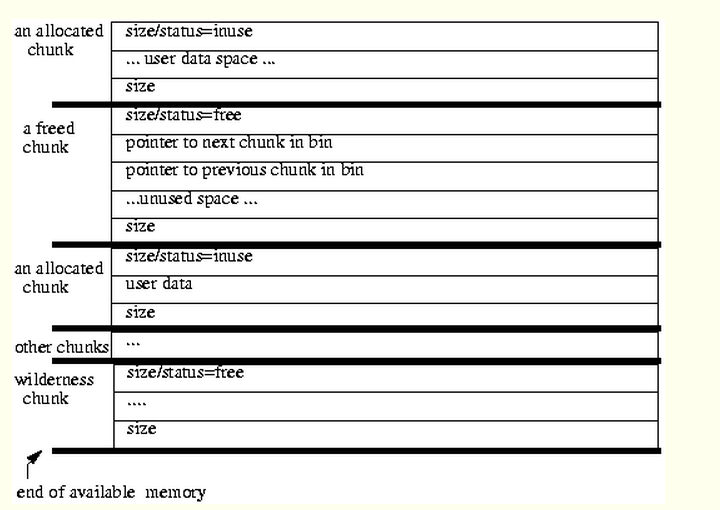
\includegraphics[width=14cm,height=14cm]{imagenes/boundary.png}

Binning

Los pedazos de memoria disponibles se agrupan en contenedores, los mismos agrupados por tamaño.  La búsqueda de pedazos disponibles se realiza buscando el pedazo más pequeño que mejor le quede al requerimiento del proceso. (smallest-first, best-fit order).



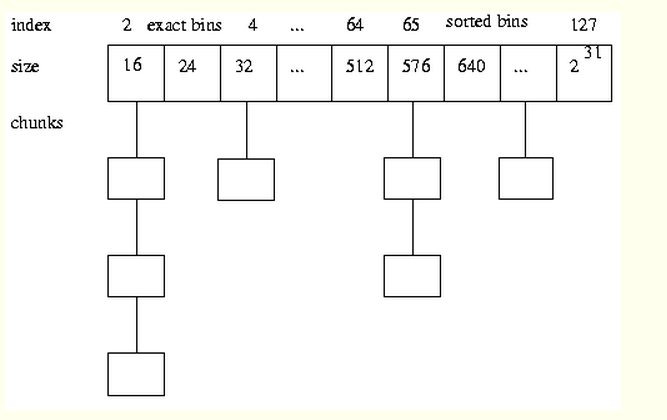
\includegraphics[width=14cm,height=9cm]{imagenes/binning.png}

En las versiones más recientes los pedazos se ordenan dentro de los contenedores, se ordenan por tamaño y por edad.

Entonces en general los pedazos libres se juntan con sus vecinos libres y se meten en un contenedor que los ordena y los dispone según se requiera.
Thus, the general categorization of this algorithm is best-first with coalescing: Freed chunks are coalesced with neighboring ones, and held in bins that are searched in size order.
En sistemas operativos de 32 bits el pedazo de memoria más pequeño que se puede ofrecer a la memoria virtual es de 16 bytes, en los de 64 bits el más pequeño es de 24 bytes.

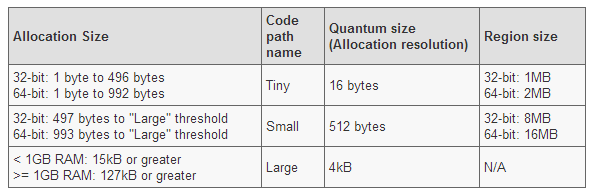
\includegraphics[width=13cm,height=5cm]{imagenes/malloc.png}




\section{Ventajas y desventajas}
	Antes de entrar en detalle acerca de las ventajas y desventajas de implementar un algoritmo de recolección de basura en C, es necesario entender que no todo programa en C se comporta de igual manera. Muchas de las ventajas y desventajas detalladas a continuación pueden o no cumplirse para cierto programa. Hay varios factores que influyen en esto: la técnica de gestión manual de memoria (malloc/free), la estructura de datos, la complejidad del programa, entre otros.
	Para los siguientes puntos, se tomara en cuenta el uso de la librería más común para recolección de basura en C, la librería Boehm-Demers-Weiser Garbage Collector o Boehm GC.
\subsection{Performance}
	Los efectos de un garbage collector, como el Boehm GC, en un programa en C pueden traer efectos variados en cuanto a la performance. Para programas pequeños que utilizan poca memoria, la implementación de un GC es probablemente innecesaria, ya que el GC requiere de un cierto espacio libre en el heap para no tener que recoger basura después de cada asignación en memoria. Ya que algunos garbage collectors expanden el heap en espacios relativamente grandes, es probable que para estos programas, parte de esa memoria nunca sea utilizada. Esto no es del todo cierto para programas con estructuras más grandes y complejas; ya que se requiere de más memoria en el heap para las asignaciones, la memoria separada por el garbage collector será utilizada más frecuente y eficientemente.
\subsection{Desarrollo}
	Es clara la ventaja que brinda la implementación de un garbage collector en un programa en C en términos de tiempo y esfuerzo de desarrollo. Ya que C no incorpora un recolector por default, es necesario manejar la memoria manualmente. Esto significa que el tiempo que tome gestionar la memoria manualmente será proporcional al tamaño y complejidad del programa. Se estima que un 30\% hasta 40\% del esfuerzo en el desarrollo de un programa extenso se enfoca solo en la gestión de memoria. Al utilizar un garbage collector, se reduce drásticamente el tiempo de desarrollo.
\subsection{Confiabilidad y Funcionalidad}
	Es más fácil y confiable el uso de grandes estructuras de datos si un recolector de basura esta implementado. Esto a su vez nos evita el tedioso trabajo de manejar límites arbitrarios para ciertos parámetros (ejemplo: tamaño de un string) y asegura que el performance sea proporcional al tamaño del programa. Aunque se puede decir que en el mejor de los casos, si se utiliza una implementación perfecta de malloc/free, queda obsoleto el uso de librerías, pero se entiende que este caso es poco probable para proyectos exrtensos.

Dlmalloc lleva en uso desde 1987 y es la versión estándar de malloc() y free() en muchos ambientes, por lo tanto su confiabilidad es muy alta.

El debugging no es recomendable a no ser que el programador lo requiera en alguna aplicación específica.Ya que estos aumentan el numero de branches.

\section{Conclusiones}
	De lo que pudimos investigar, nos llamó mucho la atención el approach que tiene C en cuanto al manejo de la memoria. Ya que sus orígenes apuntan a un acercamiento “portable assembly”, el manejo de la memoria fue dejado únicamente al usuario. Hay varios casos de hardware y algoritmos que se pueden beneficiar de un manejo de memoria especializado, y la omisión de un recolector de basura default nos genera la ventaja de poder programar para utilizar esos dispositivos y algoritmos con total libertad.
	Adicionalmente, sabemos cuándo podremos utilizar una librería con seguridad y cuando no nos conviene utilizar una para gestionar la memoria. Ya sean proyectos pequeños o grandes con los cuales nos presentemos en el futuro, sabremos cual es el camino correcto a seguir en cuanto al manejo de la memoria en C.

En conclusión El manejo de memoria en lenguaje C es un aspecto de suma importancia para el programador, ya que a diferencia de otros lenguajes este no viene incorporado por default (Garbage Collector). Por lo que el conocimiento de librerías estándar y técnicas para manejar memoria es primordial cuando se trabaja con este lenguaje

\end{document}































